\documentclass{article}
\usepackage{graphicx}
\usepackage{listings}
\usepackage{minted}
\usepackage[margin=1in]{geometry}

\begin{document}

\title{ELCT 432 Quiz 6[Late Submission]}
\author{Jacob C. Vaught}
\date{September 19, 2023}
\maketitle

\section*{Problem Statement}
Answer the following questions:
\begin{enumerate}
    \item Plot the time-domain for transmitted and received in-phase and quadrature, IQ data versus time, PSD, IQ diagram for the signal to be transmitted in MATLAB.
    \item Determine the amount of carrier frequency offset of the SDR.
    \item Why do you need to add SYNC part to transmission?
\end{enumerate}

\section*{Solutions}

\subsection*{MATLAB Code for Analysis}
To begin with, we'll first display the MATLAB code used to perform the required operations.

\begin{minted}{matlab}
%% Step 1: Prepare the image
imageRGB = imread('gamecocks.png');
imageBW = rgb2gray(imageRGB);
numberOfRows = size(imageBW,1);
numberOfCols = size(imageBW,2);

if(1)
    figure(1); imshow(imageBW);
    title('TX: Image')
end

mt = imageBW(:);
Nsamples = numel(mt);
Tsignal = Nsamples*1/fsample;

msync = linspace(0,1,10e-3*fsample).';

inphase = [msync; 0.2*(2*double(mt)-255)/255];
quadature = zeros();
IQdataTX = inphase + 1i * quadature;

% Correct for frequency offset
fcfo=1.7e3;
t=[0:numel(IQdataRX)-1].'*1/fsample;
IQdataRX = IQdataRX.*exp(1i*2*pi*fcfo*t);
\end{minted}


\subsection*{Plotting the Time-Domain and Other Characteristics}

Firstly, we use the function `analyzeIQdata` in MATLAB to generate the plots for transmitted and received in-phase and quadrature components, IQ data versus time, Power Spectral Density (PSD), and IQ diagram.

\begin{figure}[h]
    \centering
    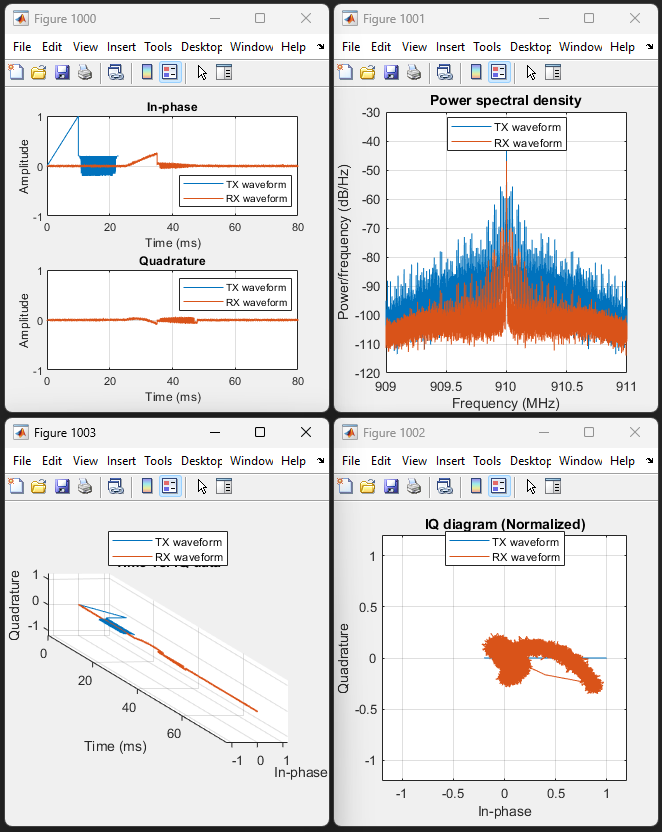
\includegraphics[width=0.8\textwidth]{Q6_P1.png}
    \caption{Plots generated using `analyzeIQdata`}
\end{figure}

\subsection*{Carrier Frequency Offset}
The carrier frequency offset of the SDR can be determined by analyzing the received IQ data. Typically, carrier frequency offsets manifest as a phase rotation in the received signal. In this specific code, the frequency offset is corrected by multiplying the received IQ data by \( \exp(1i \cdot 2 \pi \cdot f_{cfo} \cdot t) \), where \( f_{cfo} = 1.7e3 \) Hz.

\subsection*{Importance of SYNC Part in Transmission}
The SYNC part serves as a synchronization signal that aids in frame detection and alignment at the receiver. When the receiver detects this known sequence, it can more accurately align the incoming data for proper demodulation and decoding. Adding a SYNC part ensures that the receiver knows when the actual message begins, thus improving the reliability and robustness of the transmission.

\end{document}
